\section{Invereses and determinants}
\definition{Inverse function}{
    Let $T:U\to V$ be bijective.
    The \textbf{inverse of} $T$ is the unique function $T^{-1}$ that satisfies
    \begin{align*}
        T^{-1}(T(x))= x,\\
        T(T^{-1}(y))=y
    \end{align*}
    for all $x\in U, y\in V$.\\
    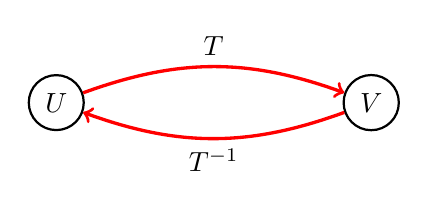
\begin{tikzpicture}
		\begin{scope}[every node/.style={circle,thick,draw}]
			\node (A) at (0,0) {$U$};
			\node (B) at (4,0) {$V$};
		\end{scope}
	
\begin{scope}[
	every edge/.style={draw=red,very thick}]
\path [->] (A) edge [bend left=20] node [above,midway]{$T$} (B);
\path [->] (B) edge [bend left=20]node [below,midway]{$T^{-1}$} (A);
\end{scope}
	\end{tikzpicture}
}
How do we know this inverse exists? We know that for each $y\in V$ there is exactly one
$x\in U$ that satisifes $T(x)=y$, so we can set $T^{-1}(y)$ to be this particular value of $x$ for each y.
This definition of the inverse sounds tautological, so let us apply this to linear transformations.
\proposition{
    Let $T:\reals^n\to\reals^n$ be a bijective linear transformation.
    Then $T^{-1}$ is a linear transformation.
}
\begin{proof}
    We want to show that for any $\vec{y}_1,\vec{y}_2\in\reals^n$, $c\in \reals$,
    $T^{-1}(\vec{y}_1+\vec{y}_2)=T^{-1}(\vec{y}_1)+T^{-1}(\vec{y}_2)$ and $T^{-1}(c\vec{y}_1)=cT^{-1}(\vec{y}_1)$.

    The trick to solving this is to use the definition for inverses and switch back and forth with $T$ and $T^{-1}$, and apply linearity of $T$.
    \begin{align*}
        T^{-1}(\vec{y}_1)+T^{-1}(\vec{y}_2) &= T^{-1}(T(T^{-1}(\vec{y}_1)+T^{-1}(\vec{y}_2)))\\
        &=T^{-1}(T(T^{-1}(\vec{y}_1))+T(T^{-1}(\vec{y}_2))) \textrm{ (as $T$ is linear)}\\
        &=T^{-1}(\vec{y}_1+\vec{y}_2).
    \end{align*}
    For scaling,\begin{align*}
        cT^{-1}(\vec{y}_1) &= T^{-1}(T(cT^{-1}(\vec{y_1})))\\
        &=T^{-1}(c(T(T^{-1}(\vec{y_1}))))\\
        &=T^{-1}(c\vec{y}_1).
    \end{align*}
\end{proof}
This means that the inverse of $T$ has a matrix representation.
If we write $T(\vec{x})=A\vec{x}$ for some matrix $A$,
then there is some matrix $B$ such that $AB=BA=I_n$.
\definition{Matrix Inverse}{
    Let $A\in M_{n\times n}(\reals)$. If there exists $B\in M_{n\times n}(\reals)$ such that
    $AB=BA=I_n$, then we say that $A$ is \textbf{invertible}, and denote $B$ is the \textbf{inverse} of $A$, written as $A^{-1}$.

}
As we have already seen, only bijective linear transformations have inverses, so that means we have more to add to That One Theorem.
\theorem{This/That One}{
    Let $A=[\vec{v}_1\ldots \vec{v}_n]\in M_{n\times n}(\reals)$, and $T:\reals^n\to\reals^n$ be the unique linear transformation satisfying $T(\vec{x})=A\vec{x}$ for all $\vec{x}\in\reals^n$.
	Then the following are equivalent.
	\begin{enumerate}
		\item $\{\vec{v}_1,\ldots,\vec{v}_n\}$ form a basis.
		\\ $\vdots$
	\end{enumerate}
	
	\begin{thatonethmlist}
		\item $T$ has an inverse $T^{-1}:\reals^n\to\reals^n$.
		\item $A$ is invertible.
	\end{thatonethmlist}
}